\section{梯度下降}
损失函数的优化求解可以通过梯度下降法实现,对于以下参数优化:
\begin{equation}
\theta^* = \arg \min L(\theta)
\end{equation}
其中,$L$为损失函数,$\theta$为优化参数。使用梯度下降迭代求解:
\begin{equation}
	\theta_n = \theta_{n-1} - \left. \eta \frac{\partial L)}{\partial \theta}\right|_{\theta_{n-1}}
\end{equation}

\subsection{学习率微调}
学习率$\eta$的调整是梯度下降法中重要的一环,过大、过小的学习率影响迭代求解的收敛性和效率。太小的学习率导致算法收敛太慢,过大的学习率反而导致算法发散,具体形象的描述可见图\ref{fig:learning_rate}。
\begin{figure}
	\centering
	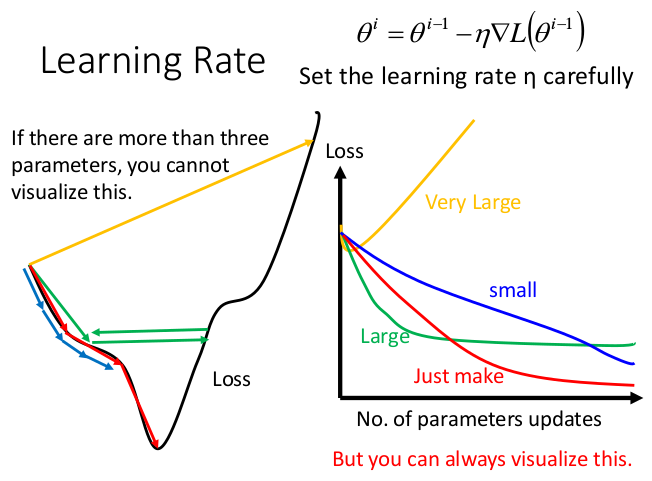
\includegraphics[scale=0.4]{pic/learning_rate}
	\caption{不同学习率下的算法迭代情况}
	\label{fig:learning_rate}
\end{figure}

通常情况下需要随着迭代次数的增加,逐渐减小学习率,主要原因是,学习的初始阶段,距离目标较远,损失函数很大,需要大的学习率,经过多轮迭代后,逐渐接近目标点,此时可以缩小学习率。

一个简单的自适应学习率可以设置为$\frac{\eta}{\sqrt{t+1}}$。

\subsubsection{adagrad}
adagrad 的权值参数设置为所有以往迭代时微分值的均方根值。权重$w$梯度表示为:
\begin{align}
g^t &= \frac{\partial (\theta^t)}{\partial w}\\
w^{t+1} &= w^t - \frac{\eta^t}{\sigma^t}g^t\\
  \\
\sigma^t &= \sqrt{\frac{1}{t+1}\sum_{i=0}^{t}(g^i)^2}
\end{align}
当$\eta^t = \frac{\eta}{\sqrt{t+1}}$时,
\begin{equation}
w^{t+1} = w^t - \frac{\eta}{\sigma^t}g^t = \frac{\eta}{\sqrt{\sum_{i=0}^{t}(g^i)^2}}
\end{equation}
\begin{myquotation}{adagrad中的疑问}
	当有大的梯度时,$g^t$导致大的步长,但分母$\sigma ^ t$导致小的步长,是否矛盾?主要可以从两个方面解释,具体参照 PPT。
	\begin{itemize}
		\item 反差
		\item 一阶微分除以二阶微分
	\end{itemize}
\end{myquotation}

\subsection{随机梯度下降法 Stochastic Gradient Descent}
一般的梯度下降法表示为:
\begin{equation}\label{eq:gd}
L = \sum _ { n } \left( \hat { y } ^ { n } - \left( b + \sum w _ { i } x _ { i } ^ { n } \right) \right) ^ { 2 }
\end{equation}
从式\eqref{eq:gd}中可以看出,梯度的求解需要所有样本参与计算。因此,计算是相对比较慢的。随机梯度下降法则是遇到一个样本,则对权重进行更新,见式\eqref{eq:sgd}因此,梯度更新相对是比较快的,相对的会造成迭代的不稳定。
\begin{equation}\label{eq:sgd}
L ^ { n } = \left( \hat { y } ^ { n } - \left( b + \sum w _ { i } x _ { i } ^ { n } \right) \right) ^ { 2 }
\end{equation}
两者的对比如图\ref{fig:gd_vs_sgd}所示。
\begin{figure}
	\centering
	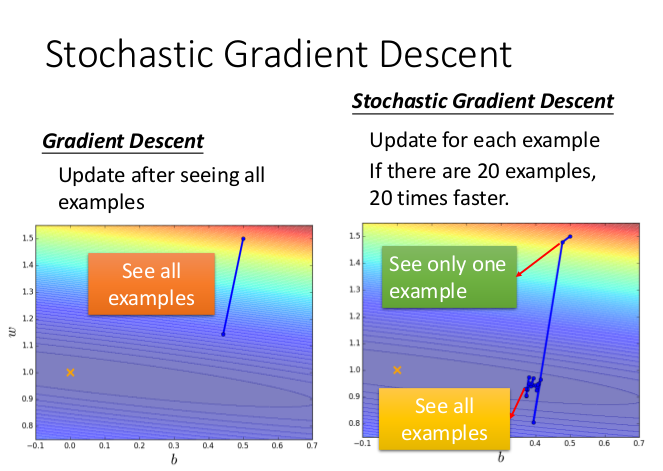
\includegraphics[scale=0.5]{pic/gd_vs_sgd}
	\caption{梯度下降法与随机梯度下降法的对比}
	\label{fig:gd_vs_sgd}
\end{figure}
\subsection{特征缩放}
特征缩放的目的是减小不同特征间尺度上的差异对迭代的影响,比如特征$x_1$的量级在100,特征$x_2$在1左右,则特征$x_1$的微小变化会对预测值有大的影响,描述见图\ref{fig:feature_scaling}。
\begin{figure}
	\centering
	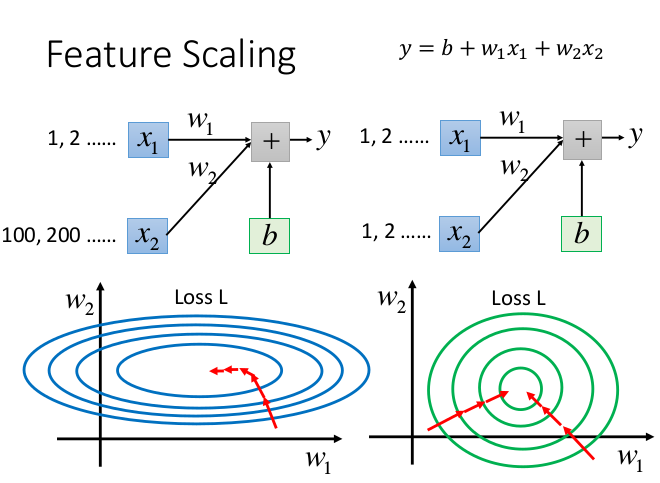
\includegraphics[scale=0.5]{pic/feature_scaling}
	\caption{特征缩放的解释}
	\label{fig:feature_scaling}
\end{figure}

常用的特征缩放方法
\begin{itemize}
	\item normalization 特征缩放后,方差为1,均值为0.见式\eqref{eq:normalization}。
	\item 归一化 0--1之间。
\end{itemize}

\begin{equation}\label{eq:normalization}
x _ { i } ^ { r } \leftarrow \frac { x _ { i } ^ { r } - m _ { i } } { \sigma _ { i } }
\end{equation}
\subsection{梯度下降数学理论}
\subsubsection{泰勒准则}
函数$h(x)$在点$x_0$附近可以展开为:
\begin{align*}
h(x) &= \sum_{k=0}^{\infty}\frac{h^k(x_0)}{k!}(x-x_0)^k\\
	&=h(x_0) + h'(x_0)(x-x_0) + \frac{h''(x_0)}{x-x0)}(x-x_0)^k
\end{align*}
\subsubsection{多元泰勒展开}
\[
h ( x , y ) = h \left( x _ { 0 } , y _ { 0 } \right) + \frac { \partial h \left( x _ { 0 } , y _ { 0 } \right) } { \partial x } \left( x - x _ { 0 } \right) + \frac { \partial h \left( x _ { 0 } , y _ { 0 } \right) } { \partial y } \left( y - y _ { 0 } \right)
\]
线性近似时:
\[
h ( x , y ) \approx h \left( x _ { 0 } , y _ { 0 } \right) + \frac { \partial h \left( x _ { 0 } , y _ { 0 } \right) } { \partial x } \left( x - x _ { 0 } \right) + \frac { \partial h \left( x _ { 0 } , y _ { 0 } \right) } { \partial y } \left( y - y _ { 0 } \right)
\]
以二元损失函数$L(\theta)$为例,在以$\theta=(a,b)$为圆心,一定半径$r$画圆,$r$是泰勒展开能够线性近似的条件。
\begin{align}
\mathrm { L } ( \theta ) &\approx \mathrm { L } ( a , b ) + \frac { \partial \mathrm { L } ( a , b ) } { \partial \theta _ { 1 } } \left( \theta _ { 1 } - a \right) + \frac { \partial \mathrm { L } ( a , b ) } { \partial \theta _ { 2 } } \left( \theta _ { 2 } - b \right)\\
s &= \mathrm { L } ( a , b )\\
u &= \frac { \partial \mathrm { L } ( a , b ) } { \partial \theta _ { 1 } }\\
v &= \frac { \partial \mathrm { L } ( a , b ) } { \partial \theta _ { 2 } }\\
\mathrm { L } ( \theta ) &\approx s + u(\theta_1-a) + v(\theta_2-b)\\
&(\theta_1-a)^2+(\theta_2-a)^2 \leq r^2
\end{align}
圆心$(a,b)$到圆上任意点$\theta=(\theta_1,\theta_2)$的向量可表示为:
\[
\left[ \begin{array} { l } { \Delta \theta _ { 1 } } \\ { \Delta \theta _ { 2 } } \end{array} \right] = 
\left[ \begin{array} { l }  \theta_1 -a \\  \theta_2 - b  \end{array} \right]
\]
因此,向量$\Delta \theta$与$(u,v)$的夹角为$180^。$时,$\mathrm { L } ( \theta )$取得最小值。即:
\[
\left[ \begin{array} { l } { \Delta \theta _ { 1 } } \\ { \Delta \theta _ { 2 } } \end{array} \right] = 
-\eta \left[ \begin{array} { l }  u \\  v  \end{array} \right]
\]
$\eta$的作用,调整$(\theta_1,\theta_2)$在圆上。故:
\begin{equation}
\left[ \begin{array} { l } { \theta _ { 1 } } \\ { \theta _ { 2 } } \end{array} \right] = \left[ \begin{array} { l } { a } \\ { b } \end{array} \right] - \eta \left[ \begin{array} { l } { u } \\ { v } \end{array} \right]
\end{equation}

这就解释了梯度下降法中迭代公式的原理。因此,不是权重每一步的迭代都能保证损失函数都能下降,因为,不能保证迭代步长使得在当前点处能够线性近似,形象的解释是,不合适的$\eta$使得$(\theta_1,\theta_2)$跑出了圆外。详细描述见图\ref{fig_math_of_gd}。
\begin{figure}[h]
	\centering
	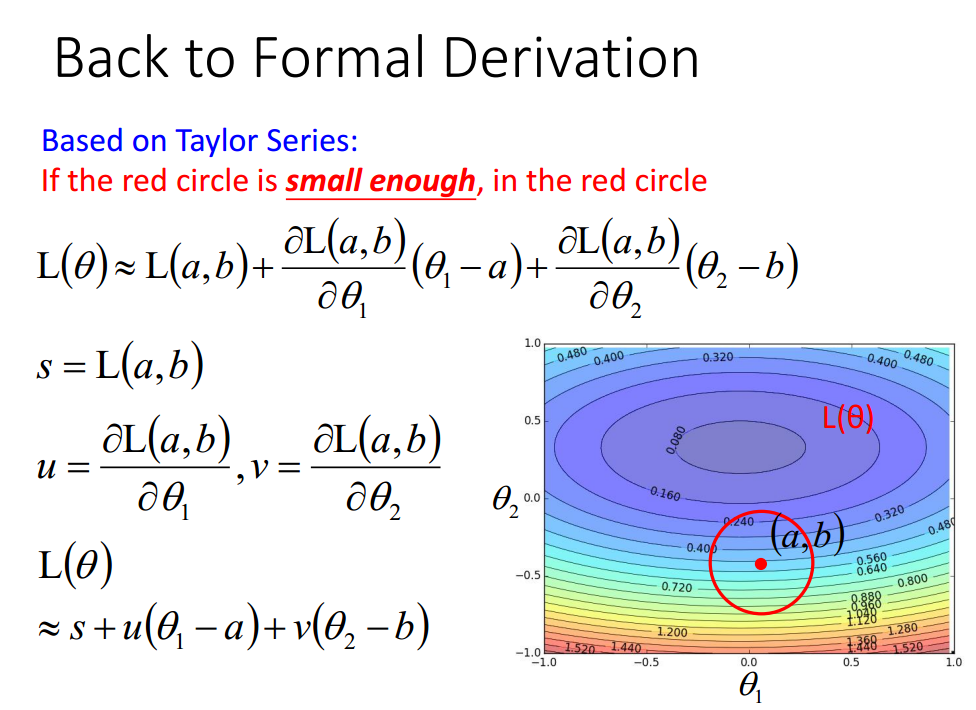
\includegraphics[scale=0.5]{pic/taylor_series}
	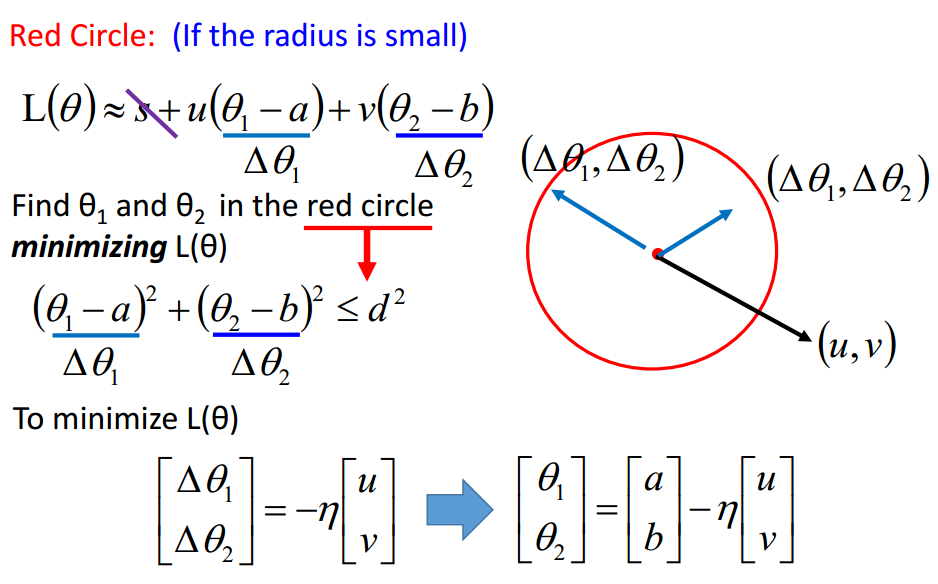
\includegraphics[scale=0.5]{pic/taylor_best}
	\caption{梯度下降法的数学解释}
	\label{fig_math_of_gd}
\end{figure}